\begin{figure}[h]
\centering
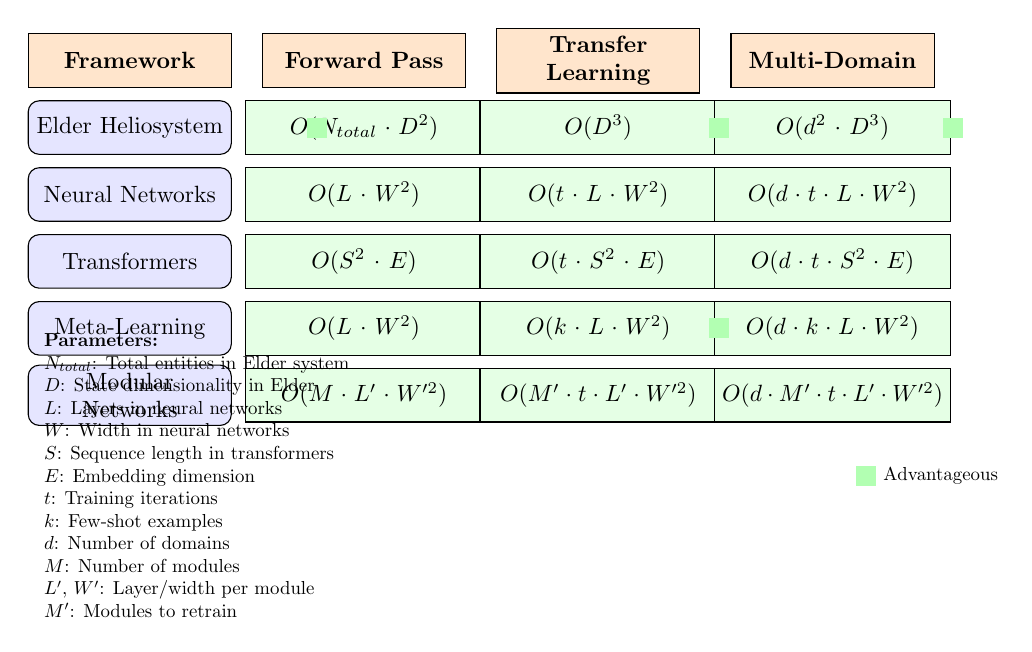
\begin{tikzpicture}[scale=0.85, transform shape]
    % Define styles
    \tikzset{
        framework/.style={draw, rounded corners, fill=blue!10, minimum width=3cm, minimum height=0.8cm, text width=2.8cm, align=center},
        operation/.style={draw, fill=gray!10, minimum width=2.5cm, minimum height=0.8cm, text width=2.3cm, align=center},
        complexity/.style={draw, fill=green!10, minimum width=3.5cm, minimum height=0.8cm, text width=3.3cm, align=center},
        thickarrow/.style={->, >=latex, thick},
        headerbox/.style={draw, fill=orange!20, minimum width=3cm, minimum height=0.8cm, text width=2.8cm, align=center, font=\bfseries}
    }
    
    % Headers
    \node[headerbox] at (0,8) {Framework};
    \node[headerbox] at (3.5,8) {Forward Pass};
    \node[headerbox] at (7,8) {Transfer Learning};
    \node[headerbox] at (10.5,8) {Multi-Domain};
    
    % Row 1: Elder System
    \node[framework] (elder) at (0,7) {Elder Heliosystem};
    \node[complexity] (elder_fwd) at (3.5,7) {$O(N_{total} \cdot D^2)$};
    \node[complexity] (elder_trans) at (7,7) {$O(D^3)$};
    \node[complexity] (elder_multi) at (10.5,7) {$O(d^2 \cdot D^3)$};
    
    % Row 2: Traditional Neural Networks
    \node[framework] (nn) at (0,6) {Neural Networks};
    \node[complexity] (nn_fwd) at (3.5,6) {$O(L \cdot W^2)$};
    \node[complexity] (nn_trans) at (7,6) {$O(t \cdot L \cdot W^2)$};
    \node[complexity] (nn_multi) at (10.5,6) {$O(d \cdot t \cdot L \cdot W^2)$};
    
    % Row 3: Transformers
    \node[framework] (trans) at (0,5) {Transformers};
    \node[complexity] (trans_fwd) at (3.5,5) {$O(S^2 \cdot E)$};
    \node[complexity] (trans_trans) at (7,5) {$O(t \cdot S^2 \cdot E)$};
    \node[complexity] (trans_multi) at (10.5,5) {$O(d \cdot t \cdot S^2 \cdot E)$};
    
    % Row 4: Meta-Learning
    \node[framework] (meta) at (0,4) {Meta-Learning};
    \node[complexity] (meta_fwd) at (3.5,4) {$O(L \cdot W^2)$};
    \node[complexity] (meta_trans) at (7,4) {$O(k \cdot L \cdot W^2)$};
    \node[complexity] (meta_multi) at (10.5,4) {$O(d \cdot k \cdot L \cdot W^2)$};
    
    % Row 5: Modular Networks
    \node[framework] (mod) at (0,3) {Modular Networks};
    \node[complexity] (mod_fwd) at (3.5,3) {$O(M \cdot L' \cdot W'^2)$};
    \node[complexity] (mod_trans) at (7,3) {$O(M' \cdot t \cdot L' \cdot W'^2)$};
    \node[complexity] (mod_multi) at (10.5,3) {$O(d \cdot M' \cdot t \cdot L' \cdot W'^2)$};
    
    % Key metrics improvement indicators
    \node[draw=none, fill=green!30, minimum size=0.3cm] at (2.8,7) {};
    \node[draw=none, fill=green!30, minimum size=0.3cm] at (8.8,7) {};
    \node[draw=none, fill=green!30, minimum size=0.3cm] at (12.3,7) {};
    
    \node[draw=none, fill=green!30, minimum size=0.3cm] at (8.8,4) {};
    
    % Legend
    \node[align=left, scale=0.8] at (1,1.8) {
        \textbf{Parameters:}\\
        $N_{total}$: Total entities in Elder system\\
        $D$: State dimensionality in Elder\\
        $L$: Layers in neural networks\\
        $W$: Width in neural networks\\
        $S$: Sequence length in transformers\\
        $E$: Embedding dimension\\
        $t$: Training iterations\\
        $k$: Few-shot examples\\
        $d$: Number of domains\\
        $M$: Number of modules\\
        $L'$, $W'$: Layer/width per module\\
        $M'$: Modules to retrain
    };
    
    % Highlights
    \node[draw=none, fill=green!30, minimum size=0.3cm] at (11,1.8) {};
    \node[scale=0.8, right=0.2cm] at (11,1.8) {Advantageous};
    
\end{tikzpicture}
\caption{Comparison of computational complexity between the Elder Heliosystem and other learning frameworks across three key operations: forward pass (standard inference), transfer learning (adapting to new tasks), and multi-domain learning (learning across multiple domains). Green highlights indicate areas where the framework offers computational advantages. The Elder system maintains comparable complexity for forward operations while achieving significant efficiency gains for transfer learning and multi-domain scenarios.}
\label{fig:framework_comparison}
\end{figure}